\chapter{The Vilpellet flight-phase segmentation}
\label{ch:vilpellet}

This chapter documents the second segmentation currently available in the analysis:
the implementation transcribed from J\'er\'emie Vilpellet's supplied inference code.
It provides a reference for reading, running and comparing that method with the
Gaussian HMM of Chapter~\ref{ch:phases}. Both methods assign transition, search and
climb to a trajectory. A choice between them for subsequent phase-conditioned
transport measurements remains open.

The probabilistic foundations are those of Section~\ref{sec:hmmtheory}: the joint law
in Eq.~\eqref{eq:hmmjoint}, Viterbi decoding in Eq.~\eqref{eq:viterbi-recursion}, and
Baum--Welch estimation in Eq.~\eqref{eq:baumwelch}. Here the observations are binary
triples and the emission law is categorical. The present implementation performs
inference under supplied parameters; it does not fit them again. The broader
phase-resolved study is described by Vilpellet et al.~\cite{vilpellet2026}, but the
operational details below follow the executable implementation and its configuration.

\section{Input, fitted parameters and admissible trajectories}
\label{sec:vilpellet-input}
The supplied inference script, \path{flight_phase_inference_minimal.py}, contains fixed
emission, transition and initial-state probabilities. The parameter provenance
recorded with the port identifies a Baum--Welch fit to 2019 paraglider flights from
four Alpine take-off sites. Those parameters are transferred unchanged to the present
flights, including hang gliders. Only the straightness threshold is discipline-specific.
This chapter describes that transfer; it does not independently reproduce the original
training or establish that its population represents the present archive.

For the default \texttt{cleaned} input, the two segmenters receive the same retained
$(E,N,z,t)$ trajectory from Chapter~\ref{ch:dataset}. Here $z$ is the pipeline's
altitude coordinate. Each preprocessing segment is decoded separately: neither a
feature window nor a hidden-state transition crosses its boundary. The optional
\texttt{raw\_gnss} command-line input instead constructs local east, north and up
coordinates directly from GNSS positions using the first fix as origin. In that
path, vertical differences are differences of local up coordinates. Changing the
input path therefore changes the observation construction, not just the file reader.

The protocol is expressed in numbers of fixes. Its eligibility conditions are shown
in Table~\ref{tab:vilpellet-gates}. The flight-level size check precedes the
segment-level checks. The entry point first orders fixes by segment and time; the
time conditions refer to those ordered sequences. The cadence check uses the
\emph{mean} interval, not a test that all intervals are equal. Uniformity within the
default cleaned input comes from preprocessing.

\begin{table}[htbp]
\centering\small
\caption{Eligibility in the current implementation. A failed check leaves the
 affected fixes \texttt{unclassified}, with a recorded reason.}
\label{tab:vilpellet-gates}
\begin{tabularx}{\textwidth}{@{}lX@{}}
\toprule
Scope & Required condition \\
\midrule
Whole flight & At least \VilpMinFixes{} retained fixes. \\
Each segment & At least \VilpPersistenceFixes{} fixes. \\
Ordered times & Unique, strictly increasing timestamps with finite increments. \\
Mean cadence & $\overline{\Delta t}<\VilpMaxMeanDtSeconds\,\mathrm{s}$. \\
\bottomrule
\end{tabularx}
\end{table}

At a one-second cadence the flight guard corresponds approximately to an hour, but
it is a fix-count rule, not a one-hour duration threshold. Likewise, a 30-fix window
covers a different physical interval when the cadence differs from one second.
The gate rejects slower logging; it does not make all accepted cadences identical.
Consequently the two segmenters need not label the same population, even when they
start from the same cleaned archive.

\section{From geometry to three binary observations}
\label{sec:vilpellet-features}
Let $k$ index fixes within one admissible segment. With the default
\texttt{pre\_smooth} option enabled, each coordinate receives a centred Gaussian
rolling mean of \VilpPositionSmoothingFixes{} fixes, with Gaussian standard deviation
equal to one sixth of the window width. Denote the resulting coordinates by
$(\widetilde E_k,\widetilde N_k,\widetilde z_k)$. Full windows are required for this
operation, so its incomplete endpoint windows remain missing. On cleaned input this
Gaussian averaging follows the pipeline's Savitzky--Golay smoothing. Keeping it
preserves the supplied feature definition, but introduces a second smoothing stage
relative to applying the reference code directly to raw GNSS positions.

Define the incoming heading and the signed change towards the outgoing step by
\begin{align}
 \theta_k &= \operatorname{atan2}(\widetilde N_k-\widetilde N_{k-1},
                                 \widetilde E_k-\widetilde E_{k-1}),\\
 r_k &= \operatorname{wrap}_{[-\pi,\pi)}(\theta_{k+1}-\theta_k),
 \qquad
 \overline r_k=\mathcal M_{\VilpTurnSmoothingFixes}[r]_k.
 \label{eq:vilpellet-turn}
\end{align}
Here $\mathcal M_w$ denotes the centred, unweighted rolling mean over $w$ fixes,
using the available nonmissing entries at a boundary. The quantity named
\texttt{radius\_curvature\_lat\_long\_sgn} in the supplied code is this signed
\emph{angle increment}, in radians per fix. It is neither a geometric radius nor
the angular velocity of Eq.~\eqref{eq:turnrate}: it is not divided by elapsed time.
For vertical motion the implementation does divide by time,
\begin{equation}
 v_{z,k}=\frac{\widetilde z_k-\widetilde z_{k-1}}{t_k-t_{k-1}},
 \qquad \overline v_{z,k}=\mathcal M_{\VilpPersistenceFixes}[v_z]_k.
 \label{eq:vilpellet-vertical}
\end{equation}
This finite-difference velocity is computed for the segmenter; it is not taken from
the preprocessing pipeline's stored vertical-velocity column.

The observation at fix $k$ is the ordered triple
$\mathbf y_k=(B^{\rm straight}_k,B^{\rm up}_k,B^{\rm sign}_k)$.
With $\beta=\VilpBetaPersistence$ and straightness threshold $a$, its first two bits are
\begin{align}
 I_k &= \mathbf 1\{-a<\overline r_k<a\},\nonumber\\
 B^{\rm straight}_k &= \mathbf 1\{\mathcal M_{\VilpPersistenceFixes}[I]_k>\beta\},
 \label{eq:vilpellet-straight}\\
 B^{\rm up}_k &= \mathbf 1\{\overline v_{z,k}>0\}.
 \label{eq:vilpellet-up}
\end{align}
The configured values of $a$ are \VilpAlphaPara{} for paragliders and
\VilpAlphaHang{} for hang gliders, in radians per fix. The configuration also supplies
\VilpAlphaSail{} for sailplanes, which are not analysed in the present archive.
The straightness inequality is strict: with a complete 30-fix window, more than
90\% means at least 28 straight fixes. Positive mean ascent alone sets only one bit;
it does not assign the climb phase.

For the third bit, take the \VilpPersistenceFixes{} values of $\overline r$ in the
window from $k-15$ through $k+14$. Select the \VilpTurnSignSelected{} largest absolute
values, retaining their signs. If $n_k^+$ and $n_k^-$ count the positive and negative
members of this selected set, then
\begin{equation}
 B^{\rm sign}_k=\mathbf 1\!\left\{
 \max(n_k^+,n_k^-)\geq
 \left\lceil\beta\,\VilpTurnSignSelected\right\rceil\right\}.
 \label{eq:vilpellet-sign}
\end{equation}
Thus at least \VilpTurnSignAgreeing{} of the selected increments must turn the same
way. Keeping the largest turns reduces the contribution of almost straight steps,
whose tiny signed increments provide little directional information. A zero increment
counts as neither positive nor negative. The code reflects the increment series at
the endpoints for this operation; it does not shorten this window.

These boundary conventions are part of the implemented model. Comparisons with
missing values evaluate false, and no additional feature-edge mask is applied before
decoding. Gaussian-smoothed endpoint gaps therefore do not automatically become
unclassified fixes. On the default path the Vilpellet wrapper also does not use
\texttt{interpolated} or \texttt{z\_reconstructed} as an additional exclusion mask.
That differs from the quality masking described in Chapter~\ref{ch:phases}, even
though both methods share the same retained trajectory.

\section{A categorical HMM and its decoded labels}
\label{sec:vilpellet-decoding}
The \VilpFeatureCount{} binary indicators have \VilpObservationValues{} possible
joint values. Their lookup index is
\begin{equation}
 c(\mathbf y)=4B^{\rm straight}+2B^{\rm up}+B^{\rm sign},
 \qquad b_i(\mathbf y)=p_{i,c(\mathbf y)}.
 \label{eq:vilpellet-emission}
\end{equation}
Each component has one probability vector over all eight triples. This is a joint
categorical distribution: the implementation does not multiply three independent
Bernoulli probabilities. Within-fix dependence between the bits is represented by
that table. The usual HMM conditional independence across observations remains an
assumption, while the overlapping feature windows induce additional temporal
structure, as discussed for the Gaussian features in Chapter~\ref{ch:phases}.

\begin{table}[htbp]
\centering\scriptsize
\setlength{\tabcolsep}{4pt}
\caption{Supplied joint emission probabilities, in lookup order and rounded to
 three decimals. Printed zeros can represent small positive probabilities;
 inference uses the full values in the configuration.}
\label{tab:vilpellet-emissions}
\begin{tabular}{@{}lrrrrrrrr@{}}
\toprule
Component & 000 & 001 & 010 & 011 & 100 & 101 & 110 & 111 \\
\midrule
\VilpEmissionRows
\bottomrule
\end{tabular}
\end{table}

The component order in this chapter is $(0,1,2)=(\mathrm C,\mathrm S,\mathrm T)$.
In that order, the supplied transition matrix and initial distribution are
\begin{align}
 A&\simeq\begin{pmatrix}\VilpTransitionMatrix\end{pmatrix},
 \label{eq:vilpellet-transition}\\
 \pi&\simeq(\VilpInitialVector).
 \label{eq:vilpellet-initial}
\end{align}
Every segment starts afresh from this $\pi$. The matrix is applied per fix; its
persistence has approximately a one-second interpretation on one-second data.
Its nonzero off-diagonal entries allow all phase transitions, rather than enforcing
a transition--search--climb cycle. The initial probability of component 2 is very
small but positive. No sequence-prior modification from Chapter~\ref{ch:phases}
is applied to this model.

Component 0 places almost all emission mass on 011: not persistently straight,
positive mean ascent and persistent turn sign. Component 2 favours 100 and 110:
persistently straight motion without a persistent turn sign. Component 1 spreads
mass over the remaining turning patterns. These emission profiles motivate the
names climb, transition and search respectively. The supplied minimal script has a
naming line that exchanges climb and transition; its numeric component paths are
unaffected. The present configuration uses the ordering supported by the emission
profiles and the accompanying code documentation. Setting
\texttt{literal\_minimal\_script} reproduces the exchanged naming line. Reproducing
numeric states and choosing their behavioural names are therefore separate checks.

Viterbi computes the most probable component path using the recurrence already
derived in Eq.~\eqref{eq:viterbi-recursion}. The implementation works in probability
space and divides all state scores by their sum at each step when that sum is
positive. This common rescaling preserves the maximizing path. Ties choose the
lowest component index. The optimized three-state recursion preserves the same
arithmetic and is tested against the general recursion.

The published phase column is then obtained by a centred majority vote over
\VilpMajorityFixes{} decoded components, using partial windows at the endpoints.
Ties again choose the lowest numeric component. This post-processing can move phase
boundaries and erase short runs; the resulting sequence is generally no longer the
Viterbi-optimal path of the original HMM. Its nominal per-fix labels do not imply
independent one-second temporal resolution. The pipeline does not compute
forward--backward posterior probabilities for these final labels.

\section{Retained runs, saved products and an example}
\label{sec:vilpellet-example}
The supplied code recommends discarding the flight tail, concentrating on long runs,
and examining searches followed by a climb. The port exposes these as optional
run-selection settings. In the present configuration the tail cut and minimum run
duration are both zero, and the following-climb condition is disabled. Thus none
of these recommendations removes an otherwise decoded fix. They should not be
confused with the active eligibility gates of Table~\ref{tab:vilpellet-gates}.

A physical track is broken at a preprocessing segment change, a nonpositive time
step, or a gap exceeding 1.5 times that segment's median positive step. A phase run
also breaks whenever its label changes. The saved run duration is $t_{\rm end}-t_{\rm start}$,
and censoring flags record whether either endpoint coincides with a physical track
boundary. These flags matter when estimating duration distributions, as already
explained in Section~\ref{sec:phaseobs}.

The default archive export writes phase intervals and segment coverage under
\path{derived/segmentation/vilpellet/}. It omits the optional fix-level table.
Intervals supply the classified labels; their complement and the coverage table
identify unclassified support. Geometry remains in \path{fixes.parquet}.
By contrast, the Chapter~\ref{ch:phases} decision table also stores features, quality
masks and posterior probabilities. This storage difference is not a missing
Vilpellet segmentation: those posterior diagnostics are not produced by this decoder.

Figures~\ref{fig:vilpellet-comparison} and~\ref{fig:vilpellet-timeline} use the same
cleaned paraglider flight, \texttt{\VilpExampleFlight}, with
\VilpExampleFixes{} fixes spanning \VilpExampleDurationMinutes{} minutes.
Both methods are run on this geometry. Table~\ref{tab:vilpellet-example} reports
phase-time shares: each fix represents the interval to the next fix in the same
physical track, with the terminal fix assigned that track's median step. This
terminal-step convention differs from summing endpoint-to-endpoint run durations.

\begin{table}[htbp]
\centering\small
\caption{Phase-time shares for the worked example, as percentages of each decoder's
 represented track time, including unclassified support. Rounding can prevent an
 exact sum of 100\%. This is one illustrative flight, not an archive-wide estimate.}
\label{tab:vilpellet-example}
\begin{tabular}{@{}lrr@{}}
\toprule
Phase & Chapter 4 decoder & Vilpellet decoder \\
\midrule
Climb & \VilpExampleGaussClimbPercent & \VilpExampleVilpClimbPercent \\
Search & \VilpExampleGaussSearchPercent & \VilpExampleVilpSearchPercent \\
Transition & \VilpExampleGaussTransitionPercent & \VilpExampleVilpTransitionPercent \\
Unclassified & \VilpExampleGaussUnclassifiedPercent & \VilpExampleVilpUnclassifiedPercent \\
\bottomrule
\end{tabular}
\end{table}

Among the \VilpExampleCommonFixes{} fixes both decoders classify, their phase names
agree on \VilpExampleAgreementPercent\%. This measures agreement between two
algorithms, not accuracy: neither label set is an independent behavioural reference.
The larger or smaller search fraction alone cannot decide which interpretation is
more useful for the intended transport observables.

\begin{figure}[htbp]
\centering
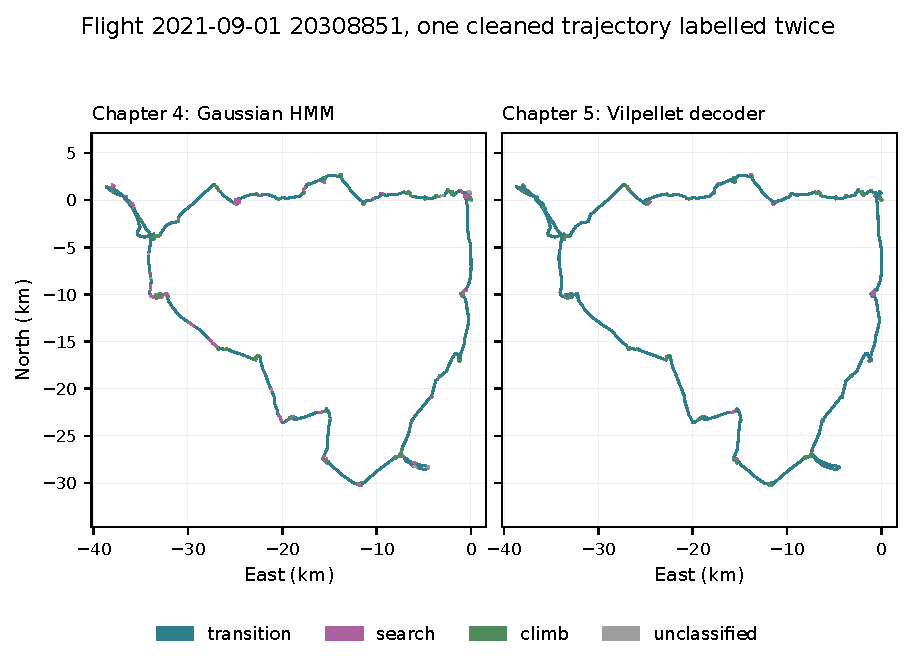
\includegraphics[width=\textwidth]{generated/ch5_vilpellet_comparison.pdf}
\caption{The same cleaned trajectory labelled by the current Chapter 4 decoder and
 the Vilpellet decoder. Coordinates and plotting limits are shared. Colour denotes
 the inferred phase, not an independently observed thermal or pilot intention.}
\label{fig:vilpellet-comparison}
\end{figure}

\begin{figure}[htbp]
\centering
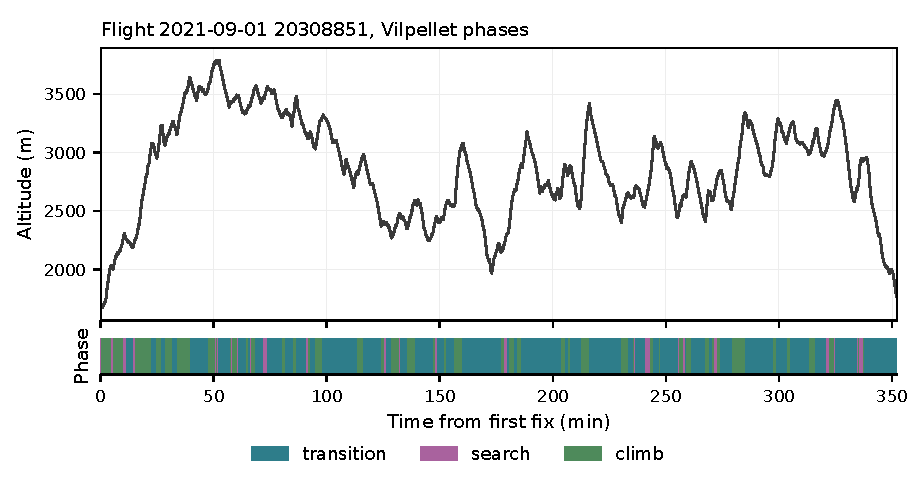
\includegraphics[width=0.93\textwidth]{generated/ch5_vilpellet_example.pdf}
\caption{Altitude and Vilpellet phase labels for the same flight. The altitude trace
 supplies physical context; sustained ascent is one input to the model and therefore
 is not independent evidence of classification accuracy.}
\label{fig:vilpellet-timeline}
\end{figure}
\FloatBarrier

\section{How to compare the two methods and where to study the code}
\label{sec:vilpellet-comparison}
Several differences can affect a phase-conditioned measurement: the continuous versus
binary observation representation; fitted versus transferred parameters; a ten-second
decision grid versus per-fix inference; quality masking versus binary boundary
conventions; and the additional majority vote. The Vilpellet cadence and flight-size
gates also remove support that the Chapter~\ref{ch:phases} decoder may classify.
Comparison therefore needs both the common classified support and each method's
coverage on the original eligible archive.

The reference-equivalence tests compare observation triples, numeric Viterbi paths
and majority-smoothed paths on synthetic and real GNSS trajectories. They test the
transcription under common inputs and deliberately check numeric components before
behavioural renaming. They do not assert that cleaned and raw inputs give the same
labels, or that a transferred model is behaviourally accurate. The same limitation
applies to the full thermal-viewer cache audit: identical outputs after a code
optimization establish computational stability, not a new validation of flight phases.

A choice between the two segmentations should use the independently annotated
windows and held-out evaluation protocol of Section~\ref{sec:phasevalidation},
reporting phase confusion, boundary behaviour and abstention alongside sensitivity
of the intended physical observables. It should also examine how smoothing,
fixed-length windows and majority voting affect apparent run durations. The geometric
sojourn law in Eq.~\eqref{eq:hmmsojourn} belongs to the latent Markov chain; it is not
a predicted empirical duration law for the majority-smoothed labels. Neither method
is selected as the final segmentation in this chapter.

For a code-first reading, start with
\path{configs/segmentation_vilpellet.yaml} for the exact constants. In
\path{src/soaring/analysis/segmentation/vilpellet/}, read
\texttt{features.py} for the coordinate operations and binary indicators,
\texttt{model.py} for the emission lookup, Viterbi recursion and majority vote,
then \texttt{pipeline.py} for eligibility, separate segment decoding and run
construction. \path{scripts/pipeline/segment_flights_vilpellet.py} defines the archive export.
The worked example and all parameter blocks printed here are generated by
\path{scripts/esperimenti/ch06_vilpellet_segmentation/generate_vilpellet_report.py}.
The implementation notes in \path{docs/guide/vilpellet-segmentation.md} provide a
longer operational reference. These paths distinguish the implemented protocol from
any future change to the segmentation or to its downstream use.
